\documentclass[ngerman,hyperref={pdfpagelabels=true}]{beamer}
\usepackage{etex}

% -----------------------------------------------------------------------------

\graphicspath{{img/}}

% -----------------------------------------------------------------------------

\usetheme{KIT}

%\setbeamercovered{transparent}
\setbeamertemplate{enumerate items}[ball]

\usepackage{ulem}
\usepackage[ngerman]{babel}
\usepackage[utf8]{inputenc}
\usepackage[TS1,T1]{fontenc}
\usepackage{array}
\usepackage[absolute,overlay]{textpos}
\usepackage{beamerKITdefs}
%\usepackage{graphicx}
%\usepackage{tikz}
\usepackage[loadonly]{enumitem}
\usepackage{hyperref}
\usepackage{etoolbox}
\usepackage{lmodern}
\usepackage{pgfplots}
\usepackage{amssymb}
\usepackage{stmaryrd}
\usepackage{listings}
\usepackage{pgffor}

\lstset{frame=tb,
        basicstyle=\scriptsize, %\ttfamily,
        numbers=left,
        numberstyle=\scriptsize,
        numbersep=5pt,
        tabsize=4,
        captionpos=t,
        language=Java,
        breaklines=true,
        breakatwhitespace=false,
        escapeinside={\%*}{*)},
        columns=flexible,
        emph={},
        emphstyle={\bfseries}%
        inputencoding={utf-8}%
        escapeinside=``%
        literate=
          {Ö}{{\"O}}1
          {Ä}{{\"A}}1
          {Ü}{{\"U}}1
          {ß}{{\ss}}1
          {ü}{{\"u}}1
          {ä}{{\"a}}1
          {ö}{{\"o}}1
          {~}{{\textasciitilde}}1
}

\newcommand{\mypath}{\rightsquigarrow}

\usetikzlibrary{trees,shapes}

\pdfpageattr {/Group << /S /Transparency /I true /CS /DeviceRGB>>}
\pdfpageattr {/Group << /S /Transparency /I true /CS /DeviceRGB>>}

\makeatletter
\patchcmd{\@maketitle}{\LARGE \@title}{\fontsize{16}{19.2}\selectfont\@title}{}{}
\makeatother


\title{Save the Robot -- Computational Geometry}
\subtitle{
February 3rd, 2016 \\ Niklas Baumstark, Samuel Groß
}


\author{Niklas Baumstark, Samuel Groß}
\institute{Institute of Theoretical Informatics}

\TitleImage[height=\titleimageht]{graphics/title}

\KITinstitute{Institute of Theoretical Informatics}
\KITfaculty{Prof. Dr. Dorothea Wagner}
%\KITfaculty{CMU Department of Computer Science}

\lstset{
basicstyle=\ttfamily\normalsize
}

\newcommand{\tikzmark}[1]{\tikz[overlay,remember picture] \node (#1) {};}
\newcommand\T{\mathcal{T}}

%\useinnertheme[shadow]{rounded}
\setbeamercolor{block title}{bg=KITblue,fg=white}
\setbeamercolor{block body}{bg=KITblue30,fg=black}

\newenvironment{mytheorem}[1]{%
\setbeamercolor{block body}{bg=KITgreen30,fg=black}
\setbeamercolor{block title}{bg=KITgreen,fg=white}
\begin{block}{Theorem: #1}}{\end{block}}

\newenvironment{mylemma}[1]{%
\setbeamercolor{block body}{bg=KITgreen30,fg=black}
\setbeamercolor{block title}{bg=KITgreen,fg=white}
\begin{block}{Lemma: #1}}{\end{block}}

\newenvironment{mydef}[1]{%
\begin{block}{#1}}{\end{block}}

\begin{document}

\setlength\textheight{7cm} %required for correct vertical alignment, if [t] is not used as documentclass parameter

\begin{frame}
  \maketitle
\end{frame}

\begin{frame}
\begin{center}
\vspace{-2em}
\only<1>{%
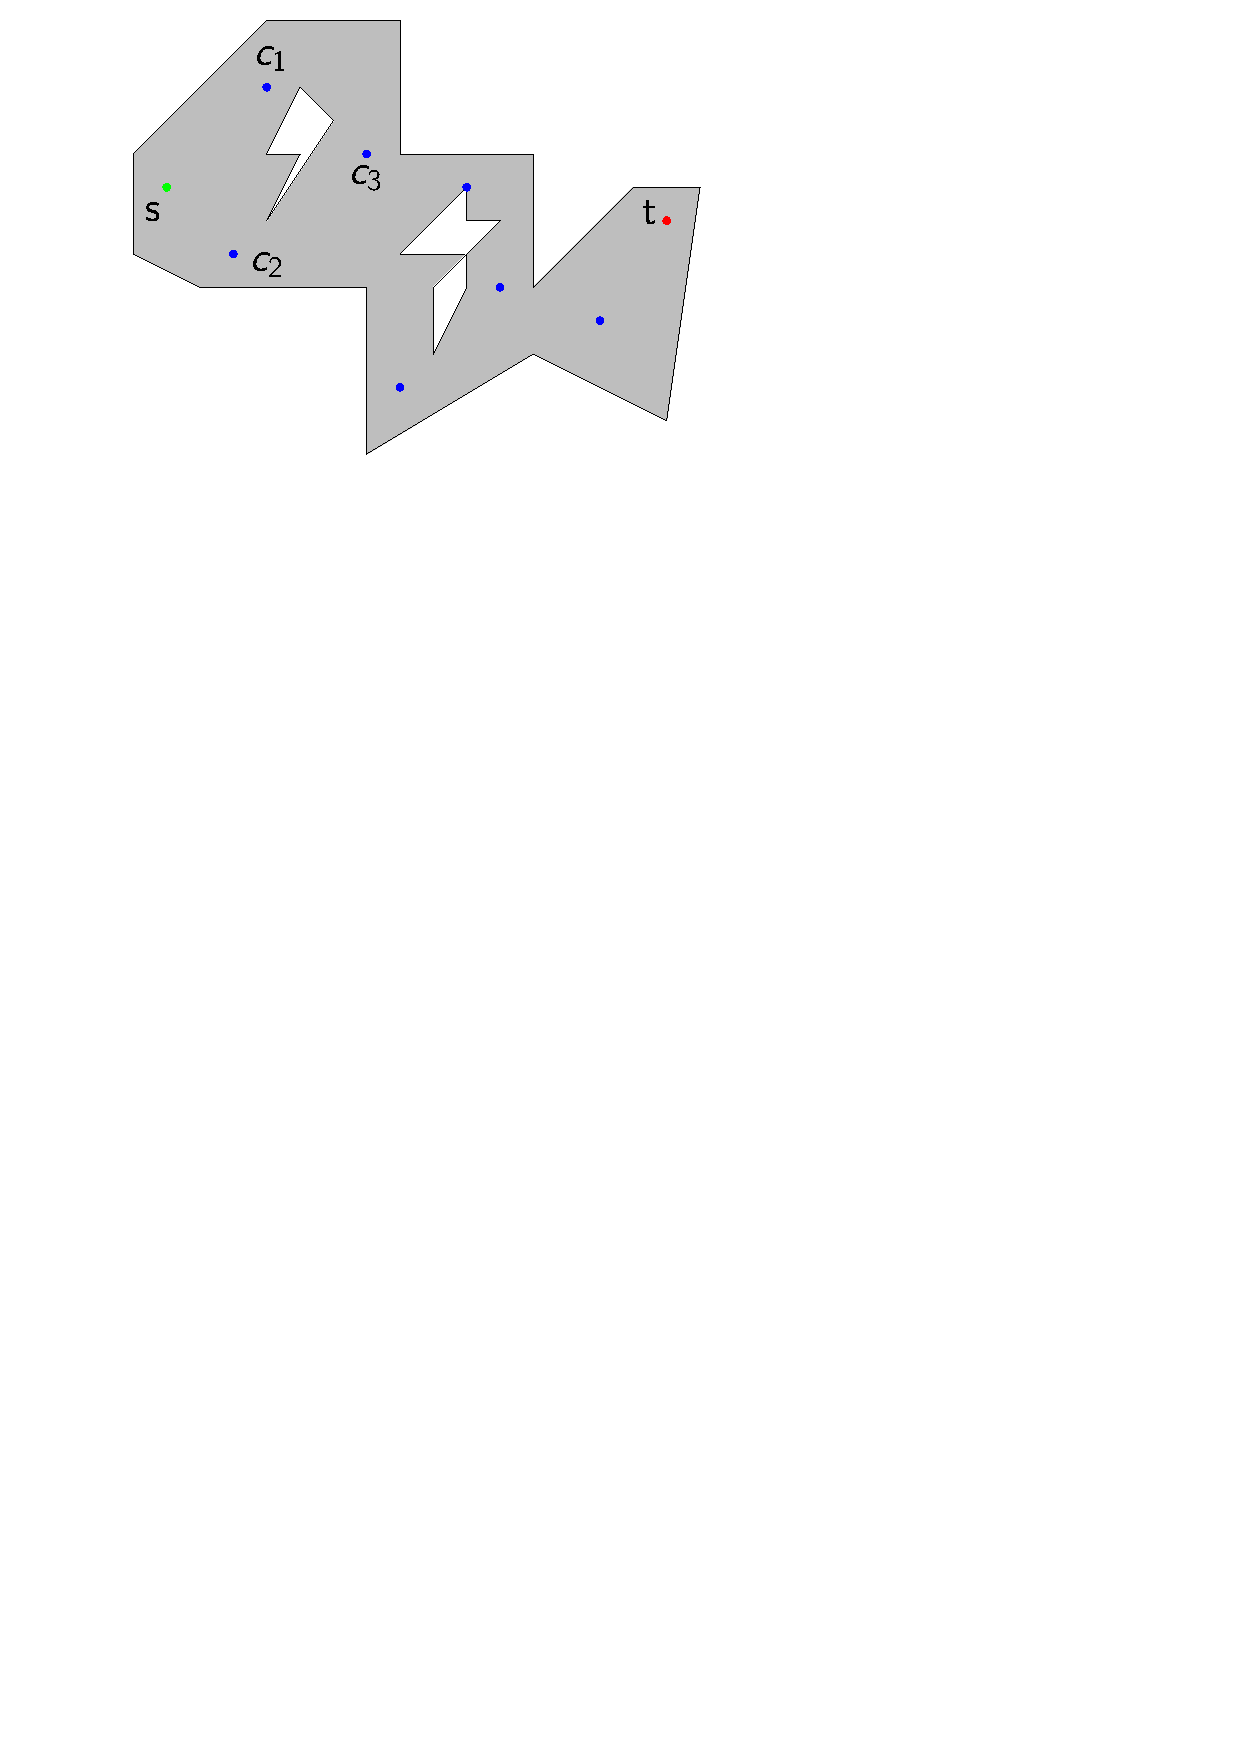
\includegraphics[page=1,height=150pt]{graphics/input1.pdf}%
}%
\only<2>{%
\includegraphics[page=2,height=150pt]{graphics/input1.pdf}%
}%
\end{center}

\begin{itemize}
\item Electric robot is in a warehouse polygon $P$, starting at green location $s$
\item Range of $r$, recharge at blue charging stations $c \in C$
\item What is the shortest path to red exit location $t$
\end{itemize}

\end{frame}

\begin{frame}{Overview}
Computing visibility graphs
\\[2em]
Computing shortest route
\\[2em]
Possible optimizations
\end{frame}

\begin{frame}{Visibility Graph}

\vspace{-1em}
\begin{mydef}{}
Given a set of points $S$ inside $P$, the \textbf{visibility graph}
of $S$ is the undirected graph $G_S = (S, E)$ with edges
$E = \{\{a, b\}\ | \  \overline{ab} \subseteq P \}$
\end{mydef}

%\begin{itemize}
%\item Let $V$ be the vertices of the polygon $P$
%\item
We are interested in the point set $S = P \cup C \cup \{s, t\}$
%\item If we know the visibility graph $G_M$, our problem reduces to the
%corresponding graph problem
%\end{itemize}
\begin{center}
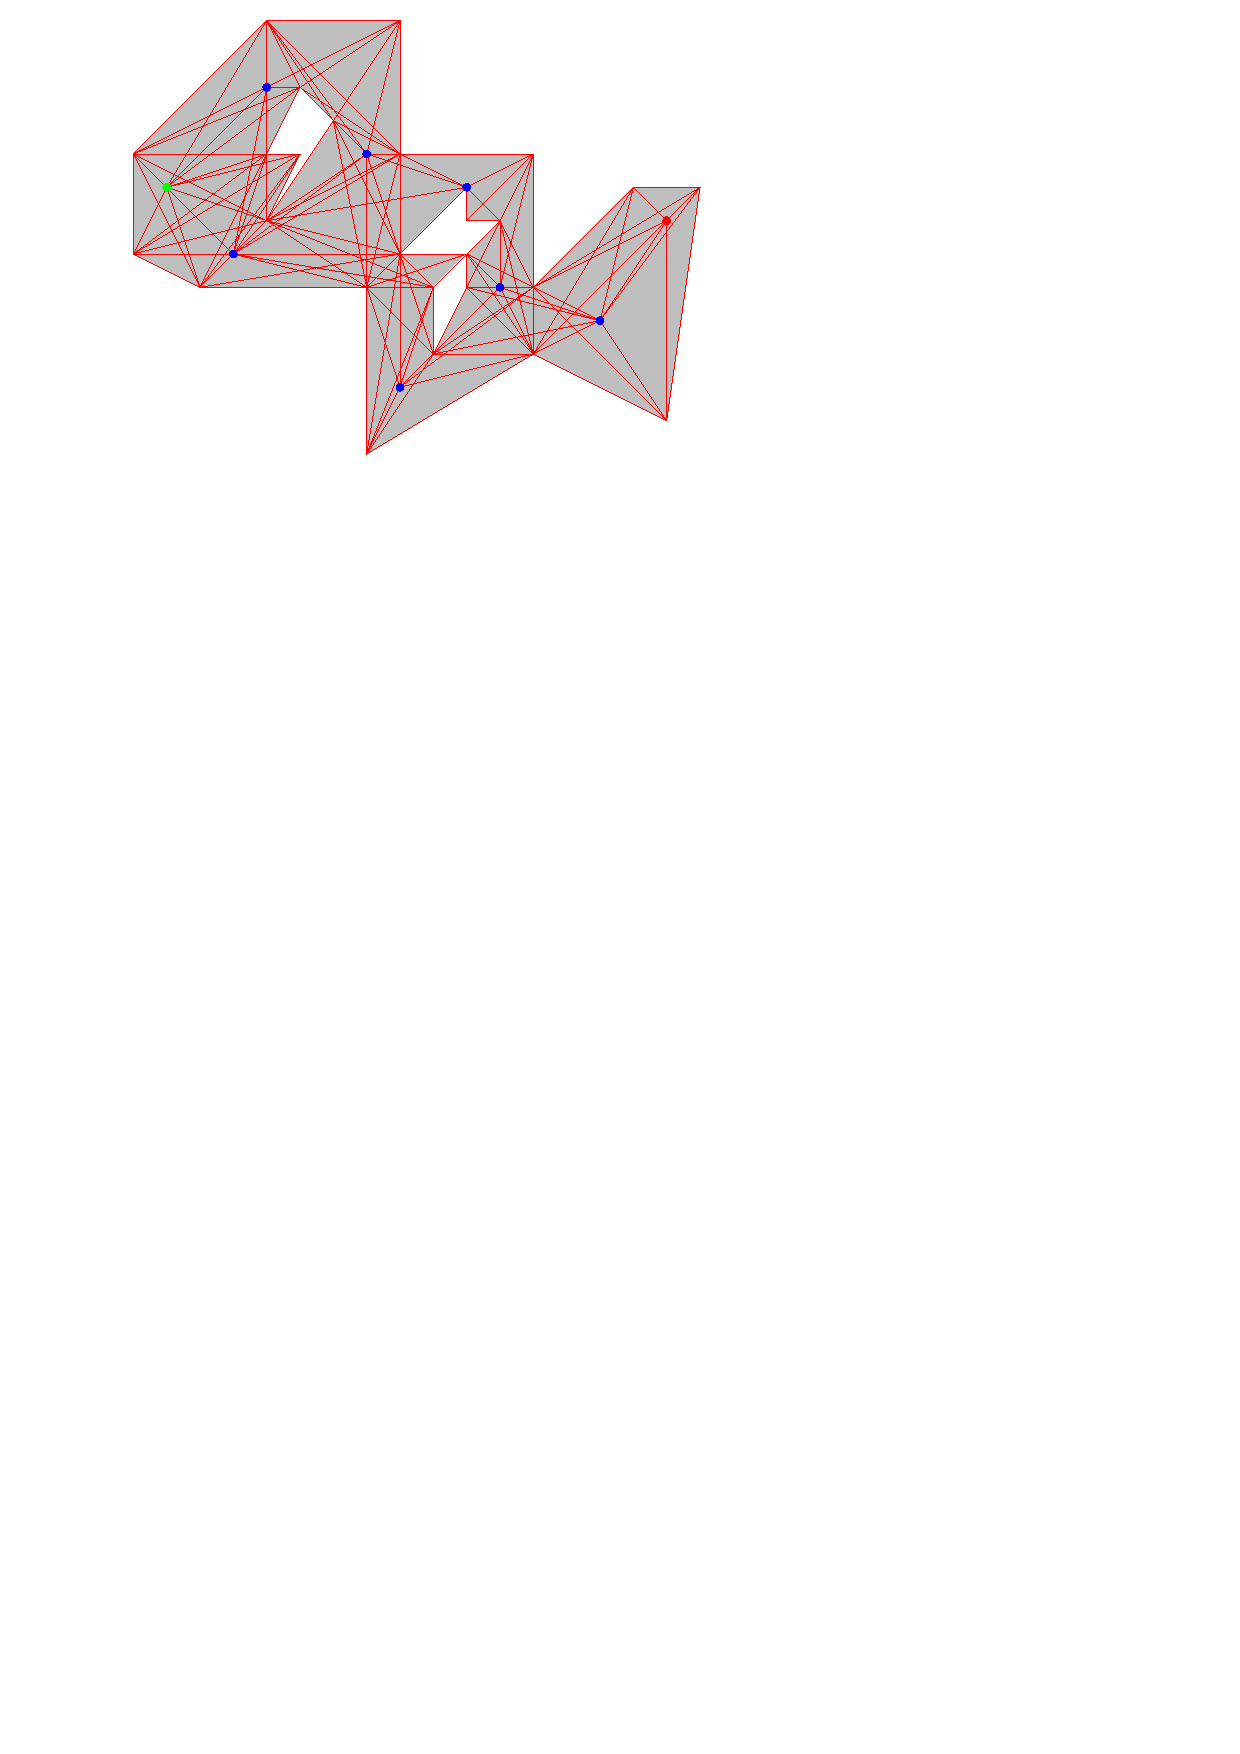
\includegraphics[height=150pt]{graphics/visibility1.pdf}
\end{center}

\end{frame}

\begin{frame}[t]{Computing $G_S$ -- First Attempt}

\vspace{-2em}
\begin{columns}
\begin{column}{0.6\textwidth}
\begin{itemize}
\item For each pair $a, b \in S$, check if $\overline{ab}$ is inside $P$
\item $\Theta(|S|^2)$ segment-in-polygon tests
\item How to check if segment $ab$ is inside $P$?
\end{itemize}
\end{column}
\begin{column}{0.35\textwidth}
\onslide<1>{%
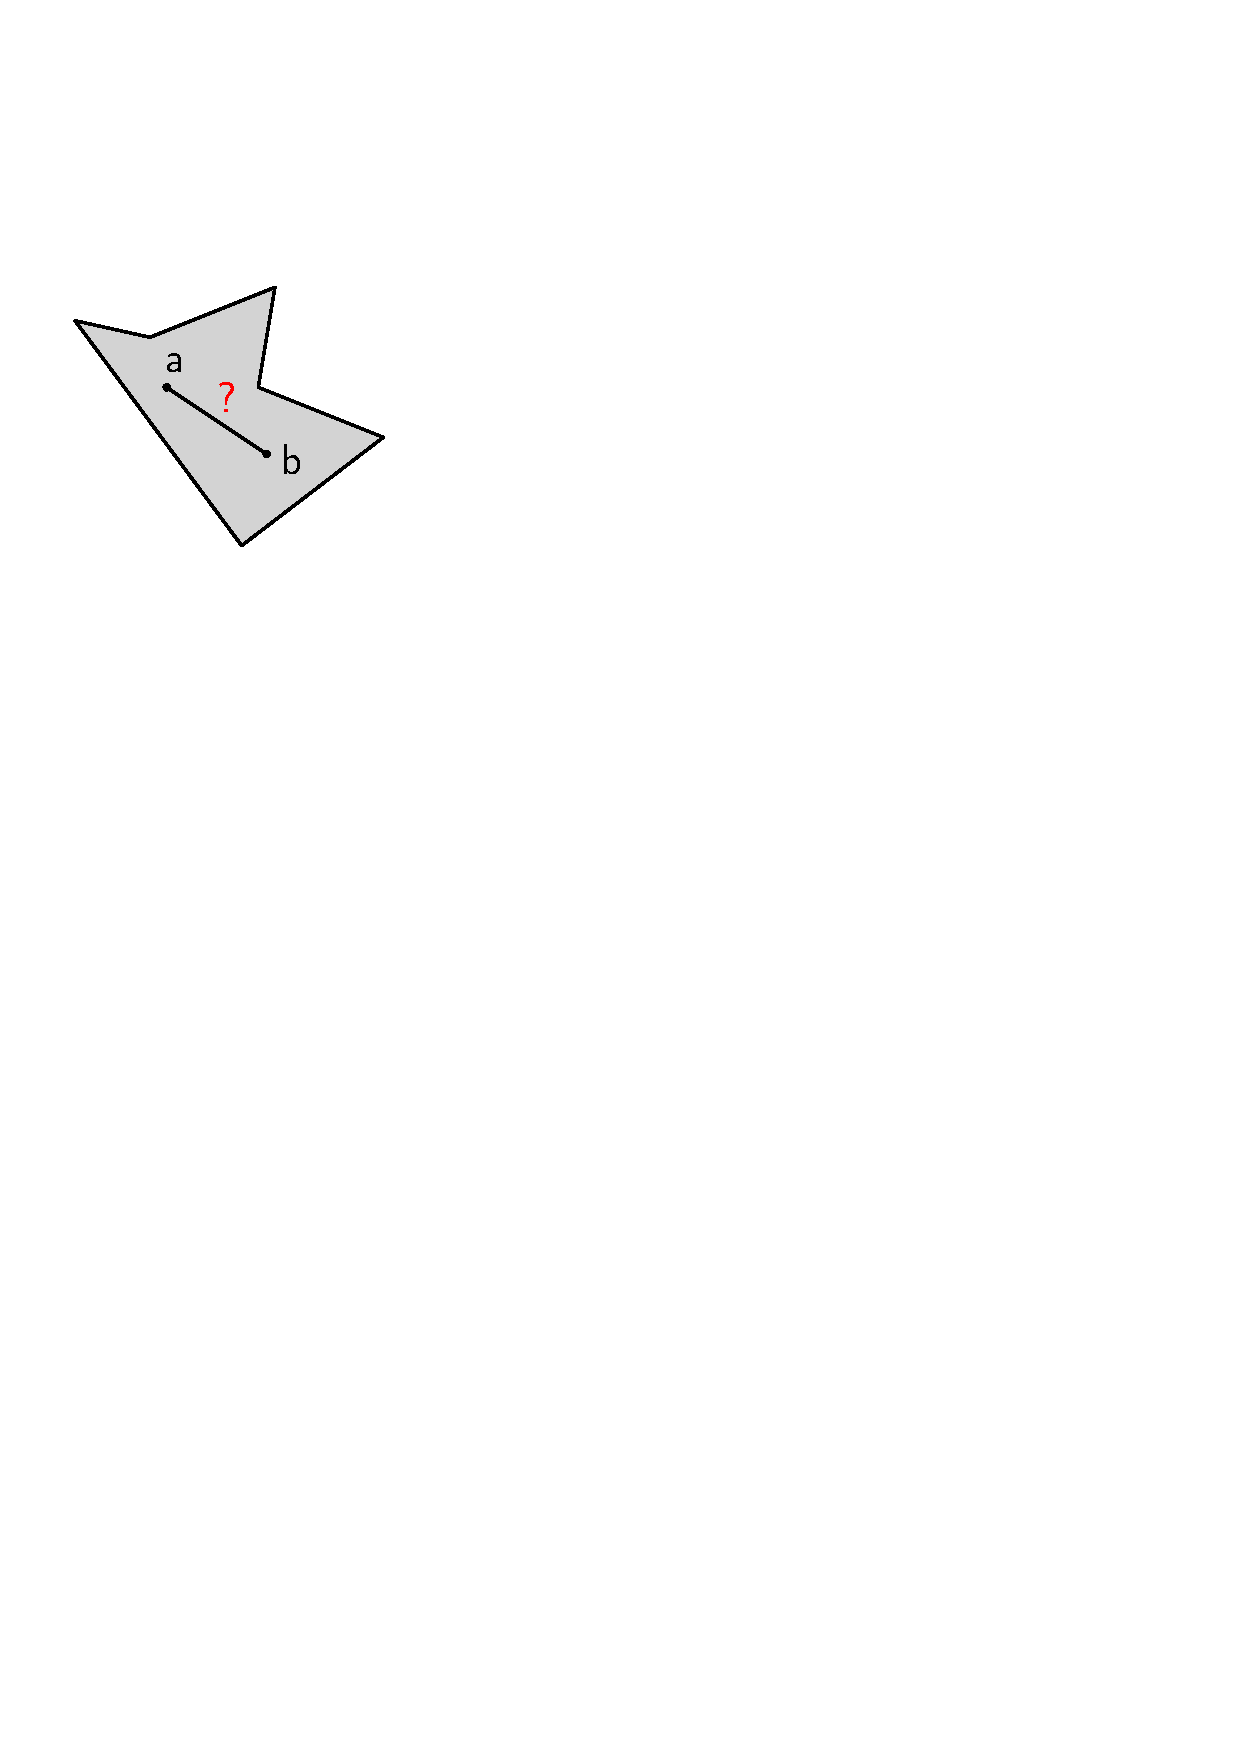
\includegraphics[page=1,height=80pt]{graphics/seg_in_poly2.pdf}%
}%
\end{column}
\end{columns}

\vspace{-1em}
\begin{center}
\begin{columns}
\begin{column}{0.48\textwidth}
\begin{enumerate}
\onslide<2->{%
\item Is there an edge $\overline{pq}$ of $P$ that intersects $\overline{ab}$ in
on the interior? \\
$\rightarrow$ output \textbf{NO}
}

\onslide<3->{%
\item Is the midpoint $(a + b)/2$ outside of $P$? \\
$\rightarrow$ output \textbf{NO}
}

\onslide<4->{%
\item Otherwise, output \textbf{YES}
}
\end{enumerate}
\end{column}

\begin{column}{0.3\textwidth}
\only<2>{%
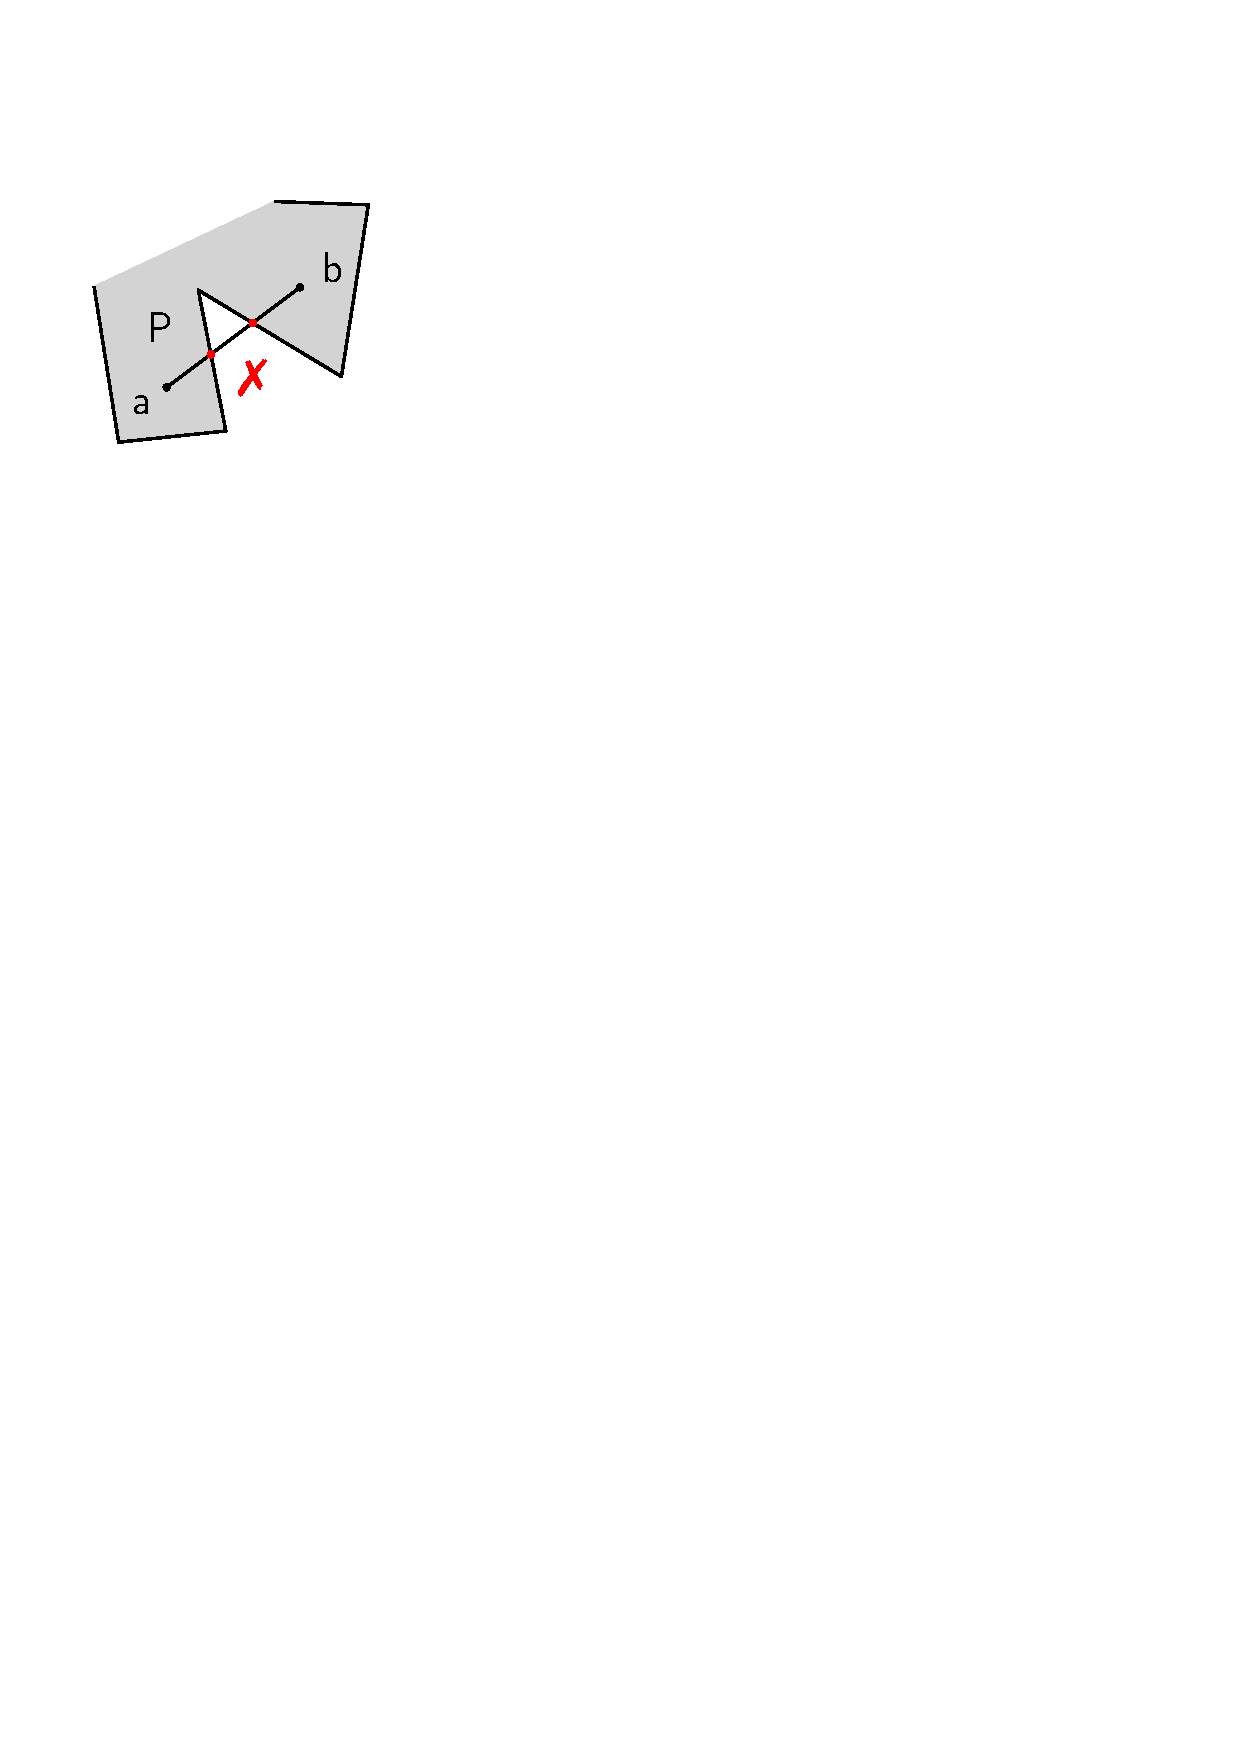
\includegraphics[page=1,height=100pt]{graphics/seg_in_poly.pdf}%
}%
\only<3>{%
\includegraphics[page=2,height=100pt]{graphics/seg_in_poly.pdf}%
}%
\onslide<4->{%
\includegraphics[page=3,height=100pt]{graphics/seg_in_poly.pdf}%
}%
\end{column}
\end{columns}
\end{center}

\onslide<5>{%
Runtime: $\Theta(|S|^2 \cdot |P|)$, dominates runtime of the algorithm
}
\end{frame}

\begin{frame}[t]{Computing $G_S$ -- Second Attempt}
\vspace{-1em}
\begin{itemize}
\item For each $a \in S$, compute points $b$ with $\overline{ab}$ inside $P$ in one pass
\item Use \textbf{Circle-Sweep}: Sort all points/vertices by their angle around $a$
\item Maintain edges of $P$ intersecting the sweep line, sorted by distance
\onslide<17>{
\item Runtime: $\Theta(|S| \cdot n \cdot \log n)$ where $n = |S| + |P|$
\item Now that we have $G_S$, how to solve the problem on a general graph?
}
\end{itemize}
\vspace{-3em}
\begin{center}
\foreach \n in {1,...,15}{%
\only<\n>{%
\includegraphics[page=\n,height=155pt]{graphics/circle_sweep.pdf}%
}%
}
\onslide<16>{%
\includegraphics[page=16,height=155pt]{graphics/circle_sweep.pdf}%
}%
\end{center}

\end{frame}



\begin{frame}{Status}
\sout{Computing visibility graphs}
\\[2em]
Computing shortest route
\\[2em]
Possible optimizations
\end{frame}

\begin{frame}{Computing shortest route}

\begin{center}
\vspace{-1em}
\only<1>{%
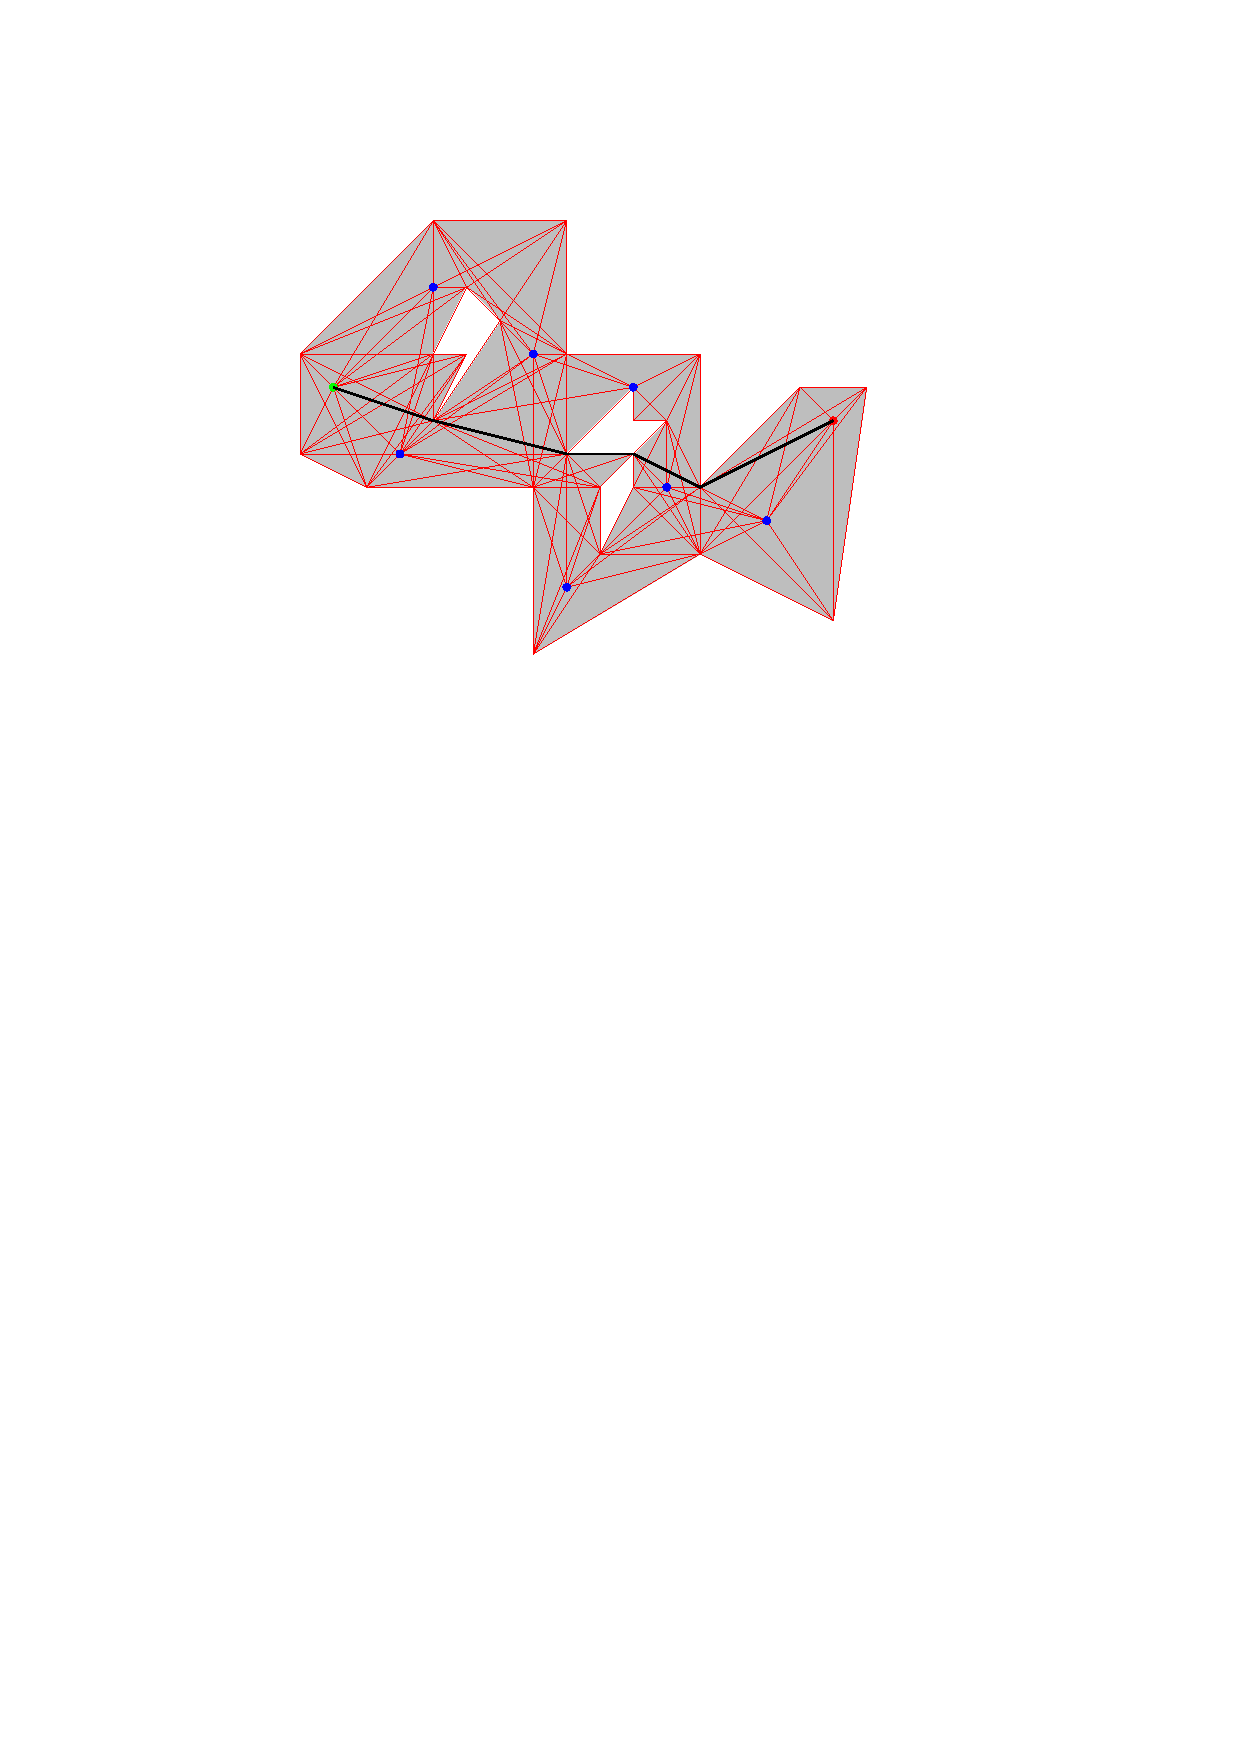
\includegraphics[page=1,height=200pt]{graphics/not_working.pdf}%
}%
\only<2>{%
\includegraphics[page=2,height=200pt]{graphics/not_working.pdf}%
}%
\end{center}
\end{frame}

\begin{frame}{Computing shortest route}

\begin{itemize}
\item Problem: How to guarantee that path includes charging stations?
\pause
\item Idea: Perform search on a reachability graph:
    \begin{itemize}
        \item Edges only between charging stations (plus start/end node)
        \item There's an edge between two nodes only if there's a path between them in the visibility graph that has a length of at most $r$
    \end{itemize}
\end{itemize}
\vspace{-2em}
\pause
\begin{center}
\includegraphics[page=10,height=160pt]{graphics/algo_basic.pdf}
\end{center}

\end{frame}

\begin{frame}{Status}
\sout{Computing visibility graphs}
\\[2em]
Computing shortest route
\begin{itemize}
    \item Computing reachability graph
    \item Computing final path on reachability graph
\end{itemize}
\vspace{2em}
Possible optimizations
\end{frame}


\begin{frame}[t]{Computing reachability graph}

\begin{itemize}
\item Compute shortest path from every charging station to all reachable charging stations
\end{itemize}

\vspace{-2em}

\begin{center}
\only<1>{%
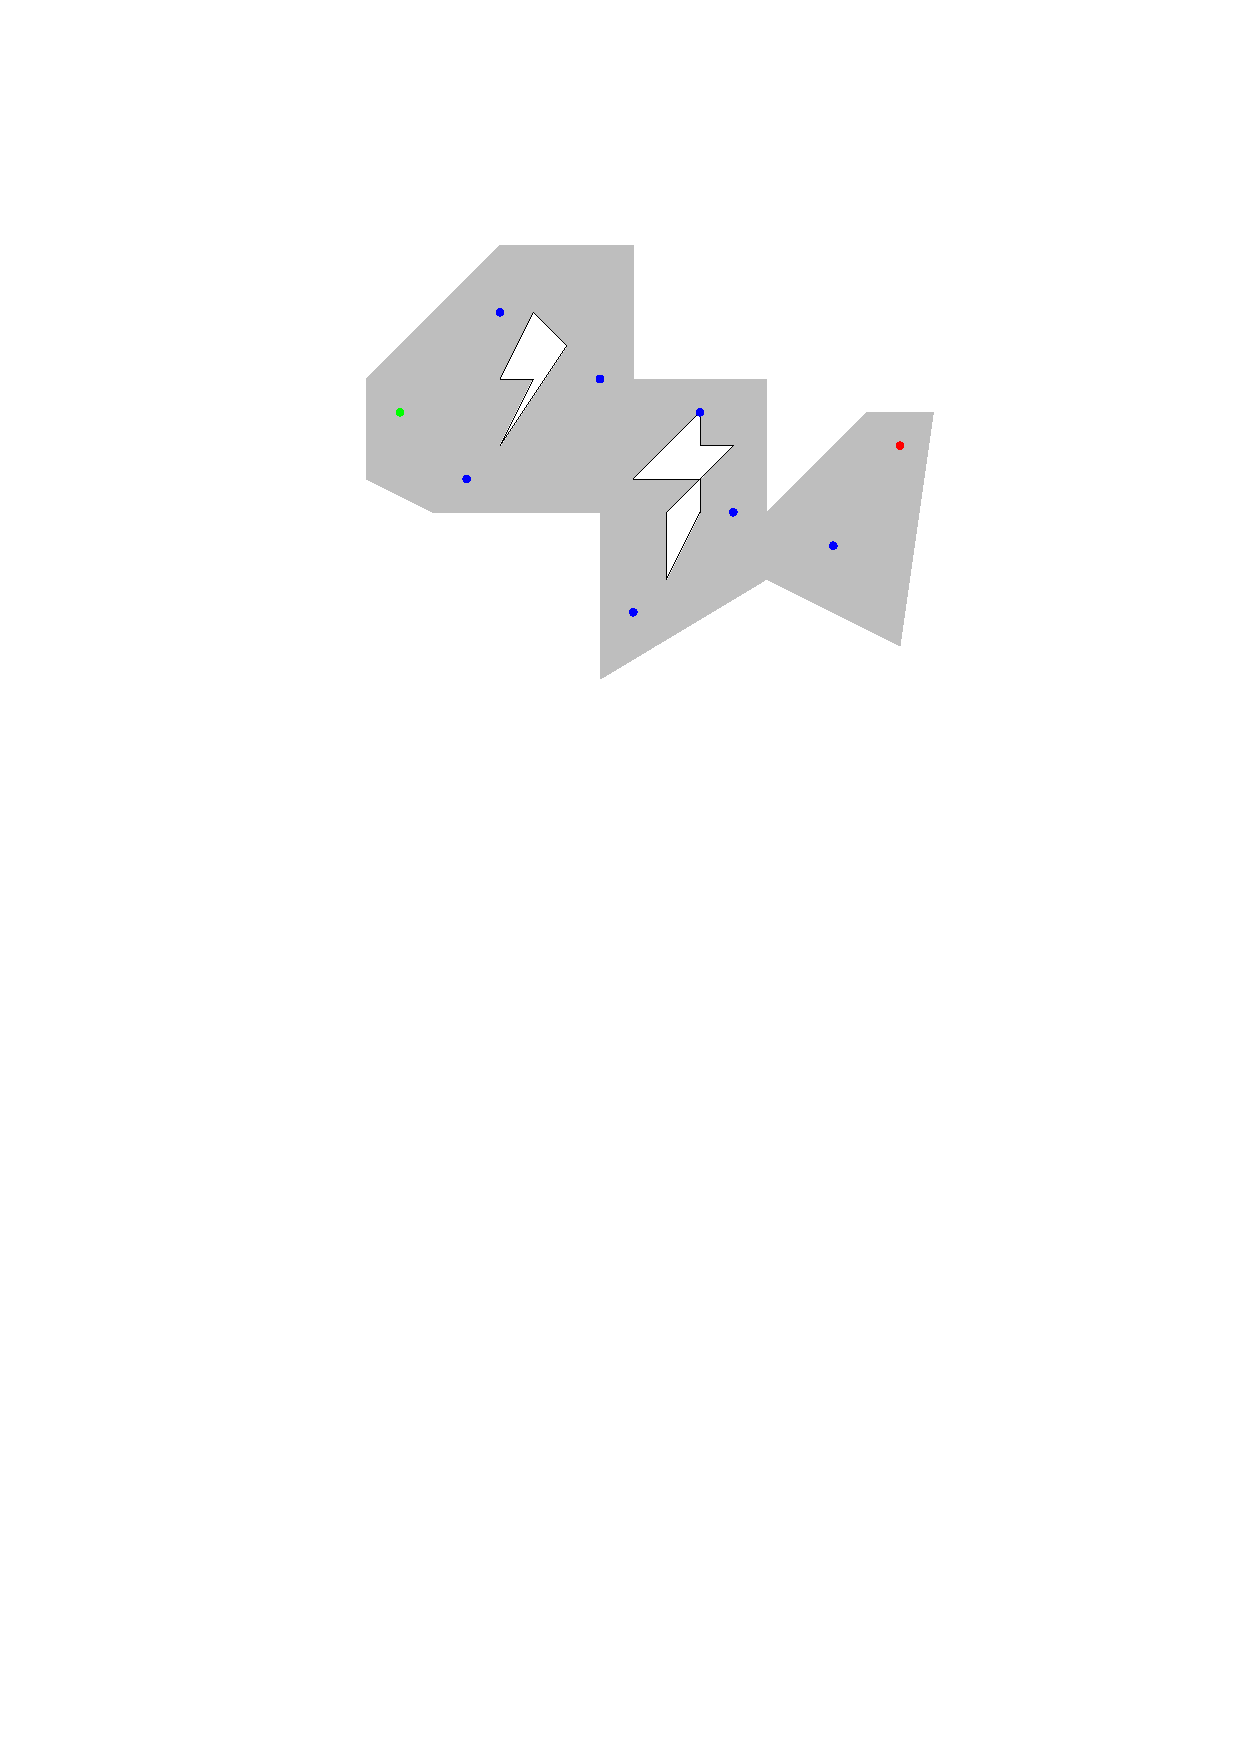
\includegraphics[page=1,height=200pt]{graphics/algo_basic.pdf}%
}%
\only<2>{%
\includegraphics[page=2,height=200pt]{graphics/algo_basic.pdf}%
}%
\only<3>{%
\includegraphics[page=3,height=200pt]{graphics/algo_basic.pdf}%
}%
\only<4>{%
\includegraphics[page=4,height=200pt]{graphics/algo_basic.pdf}%
}%
\only<5>{%
\includegraphics[page=5,height=200pt]{graphics/algo_basic.pdf}%
}%
\only<6>{%
\includegraphics[page=6,height=200pt]{graphics/algo_basic.pdf}%
}%
\only<7>{%
\includegraphics[page=7,height=200pt]{graphics/algo_basic.pdf}%
}%
\only<8>{%
\includegraphics[page=8,height=200pt]{graphics/algo_basic.pdf}%
}%
\only<9>{%
\includegraphics[page=9,height=200pt]{graphics/algo_basic.pdf}%
}%
\only<10>{%
\includegraphics[page=10,height=200pt]{graphics/algo_basic.pdf}%
}%
\only<11>{%
\includegraphics[page=12,height=200pt]{graphics/algo_basic.pdf}%
}%
\end{center}

\end{frame}

\begin{frame}{Status}
\sout{Computing visibility graphs}
\\[2em]
Computing shortest route
\begin{itemize}
    \item \sout{Computing reachability graph}
    \item Computing final path on reachability graph
\end{itemize}
\vspace{2em}
Possible optimizations
\end{frame}

\begin{frame}[t]{Computing final route}

\begin{itemize}
    \item Need one final (shortest) path computation from start to end node
    \visible<2,3>{\item Runtime: Visibility graph + $(|C| + 3)$ shortest path calculations}
    \visible<3>{\item Runtime: $$\mathcal{O}(((|C| + |P|)^2 + |C| \cdot |E|) \cdot \log(|C| + |P|))$$}
\end{itemize}

\begin{center}
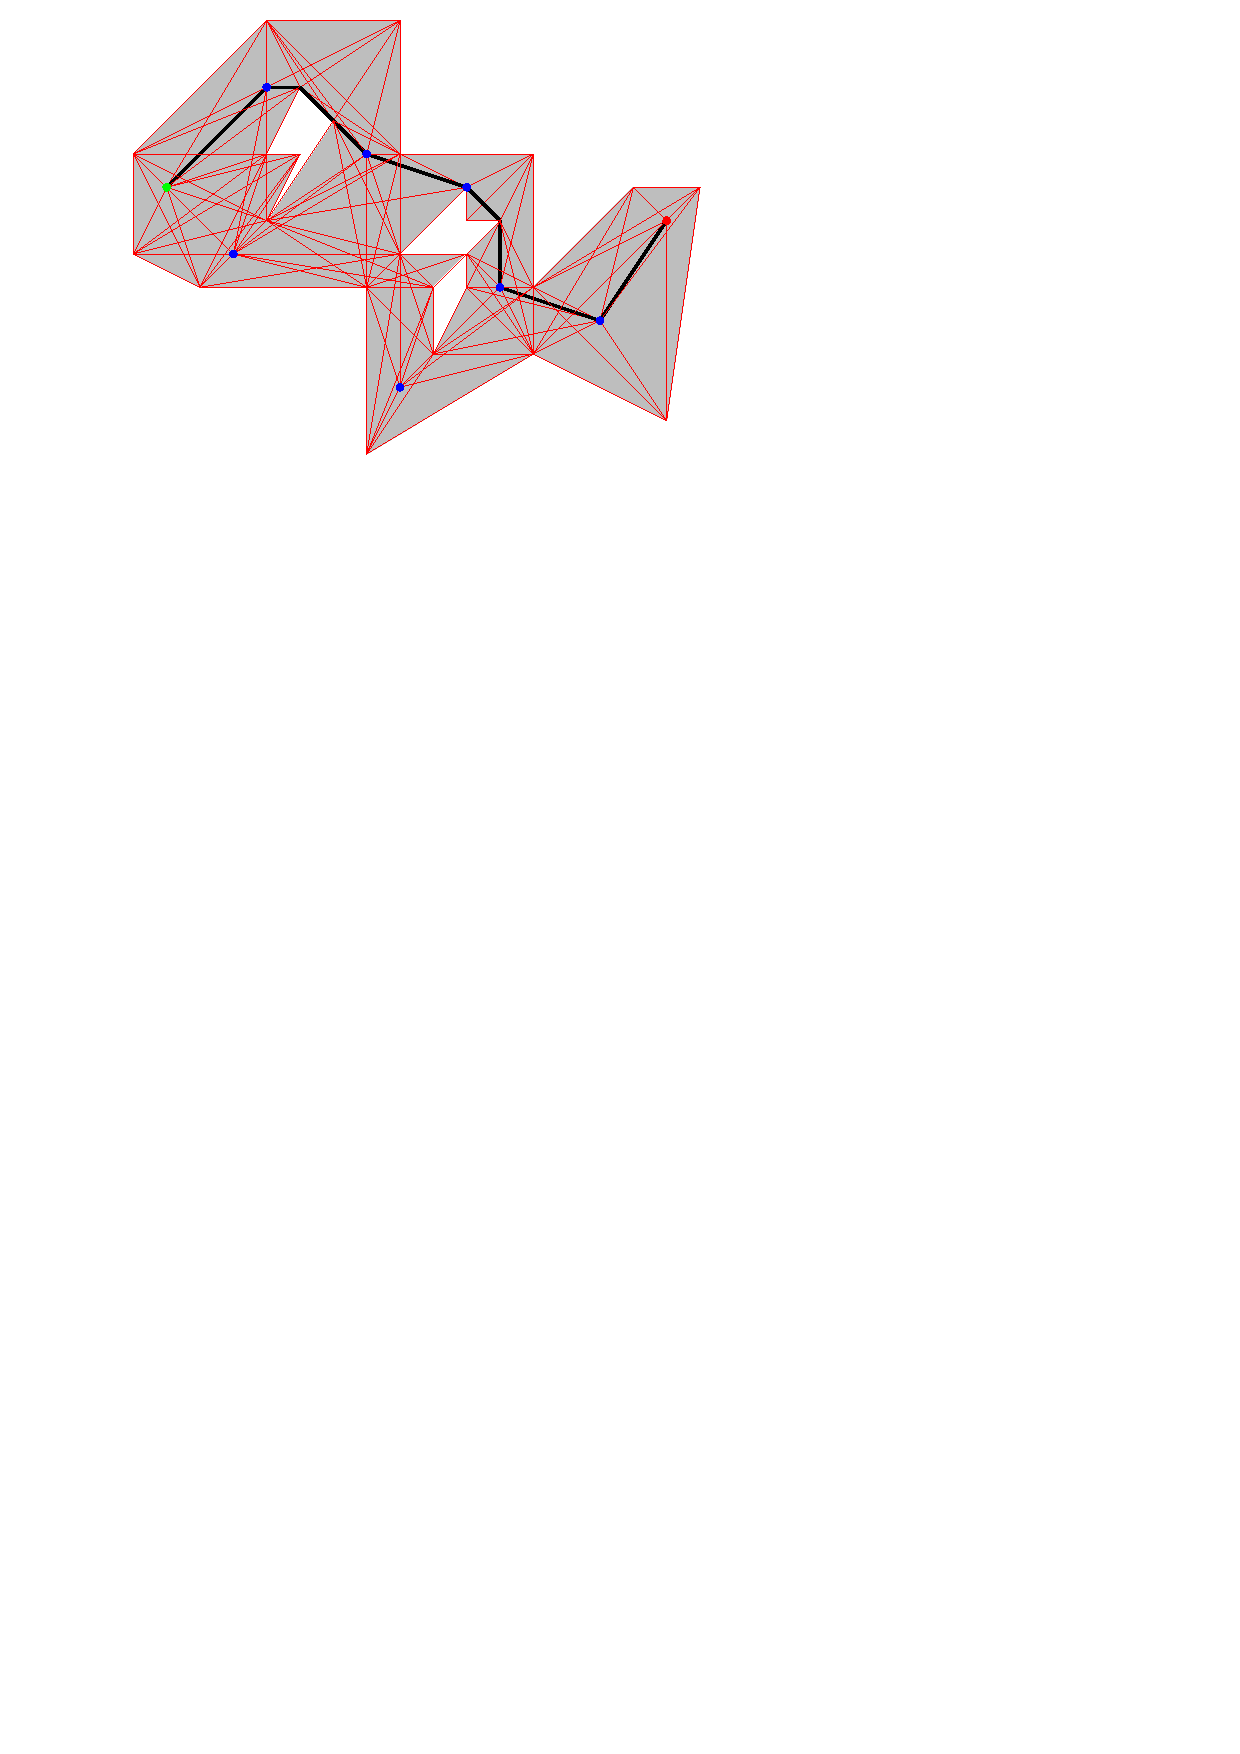
\includegraphics[page=1,height=100pt]{graphics/final.pdf}%
\end{center}

\end{frame}

\begin{frame}{Status}
\sout{Computing visibility graphs}
\\[2em]
\sout{Computing shortest route}
\begin{itemize}
    \item \sout{Computing reachability graph}
    \item \sout{Computing final path on reachability graph}
\end{itemize}
\vspace{2em}
Possible optimizations
\end{frame}

\begin{frame}[t]{Further Optimization: Problem}

\begin{itemize}
    \item Huge input set, but start and end are close together (compared to size of the input)
    \item Need to compute visibility graph for whole input set, expensive!
\end{itemize}

\vspace{2em}

\begin{center}
\only<1>{%
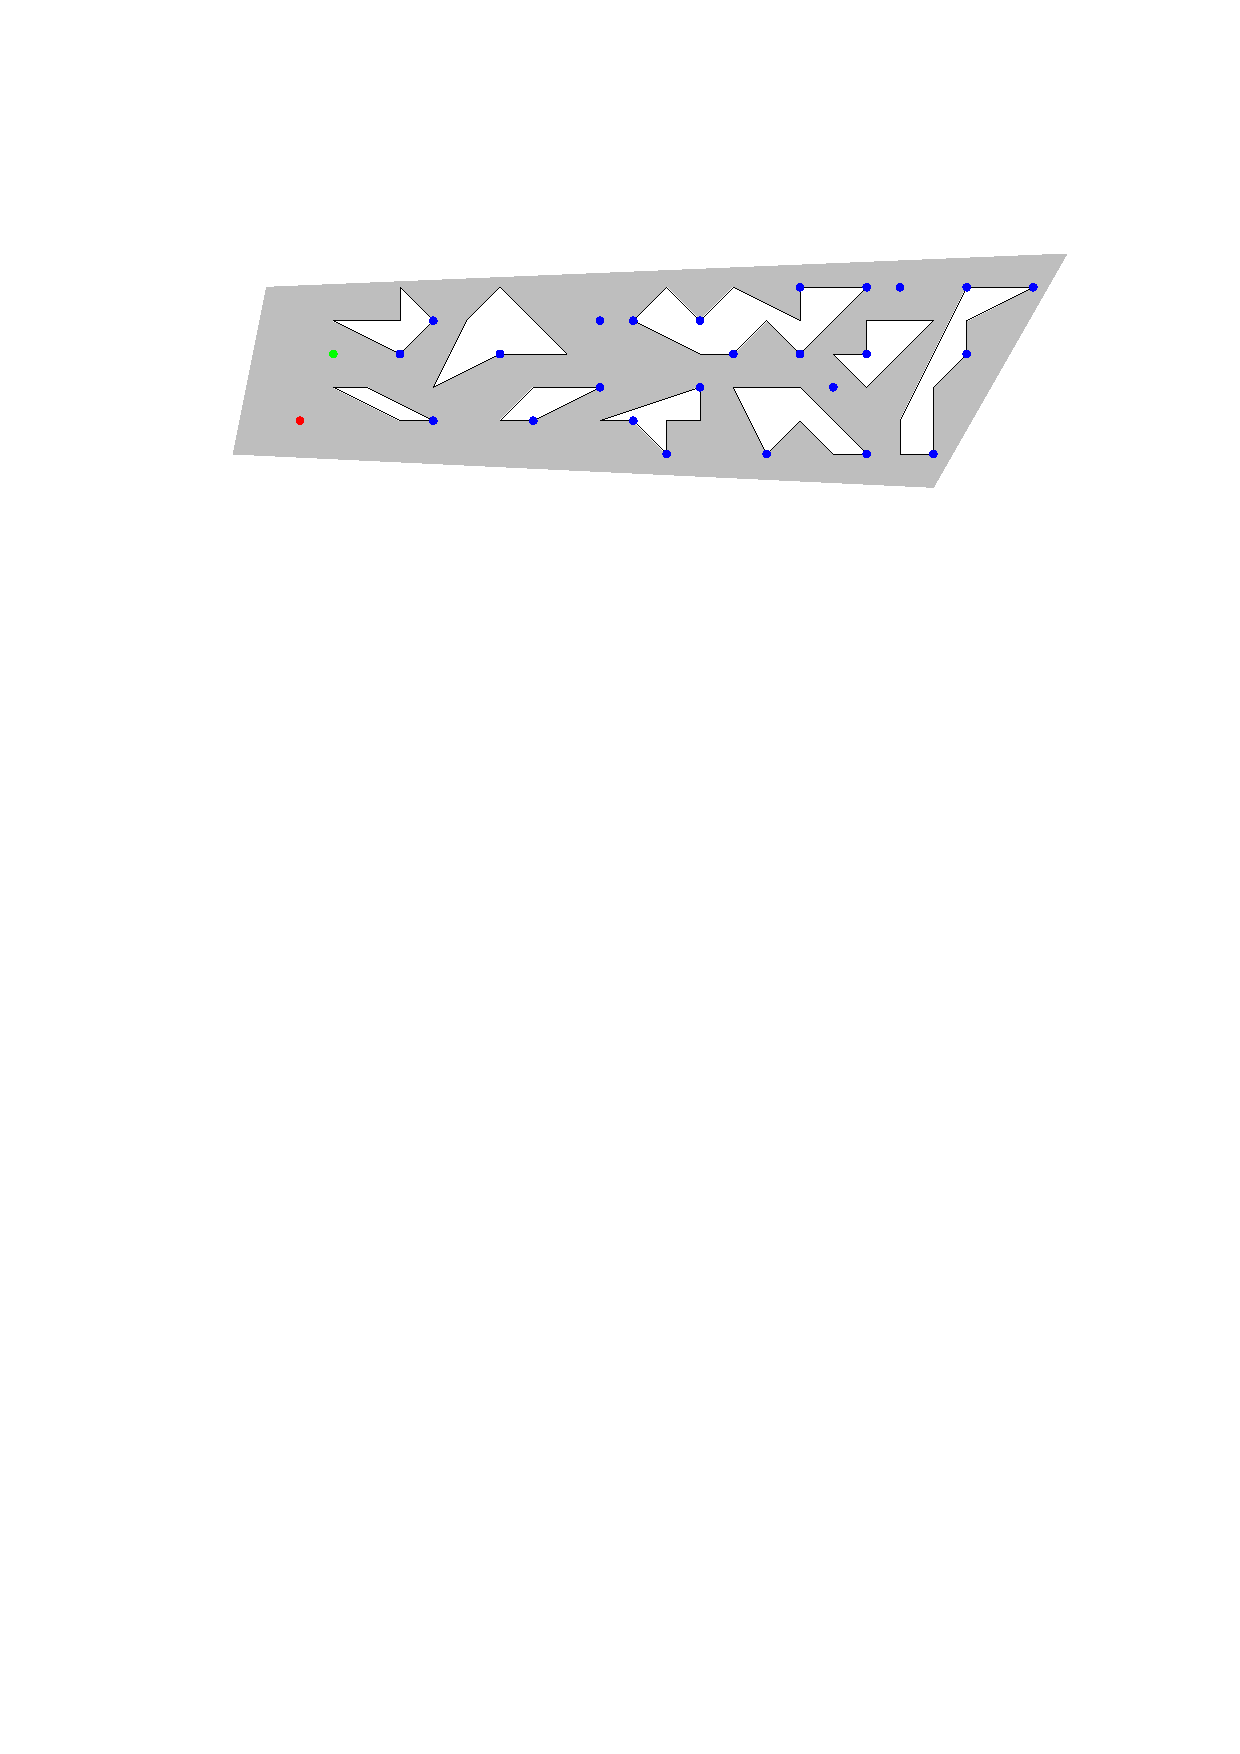
\includegraphics[page=1,height=80pt]{graphics/further_stuff.pdf}%
}%
\only<2>{%
\includegraphics[page=2,height=80pt]{graphics/further_stuff.pdf}%
}%
\end{center}
\end{frame}

\begin{frame}[t]{Further Optimization: Idea}

\begin{itemize}
    \item Compute visibility graph and shortest paths ''on-demand'':
    \begin{enumerate}
        \item Start at $s$
        \item Compute visibility graph for all nodes in radius $r$ around current node
        \item Perform shortest path search for each charging station in current radius
        \item Pick charging station with lowest distance to $s$ as next node
        \item Go back to 2. until end node $t$  found
    \end{enumerate}
\end{itemize}

\vspace{2em}

\begin{center}
\only<1>{%
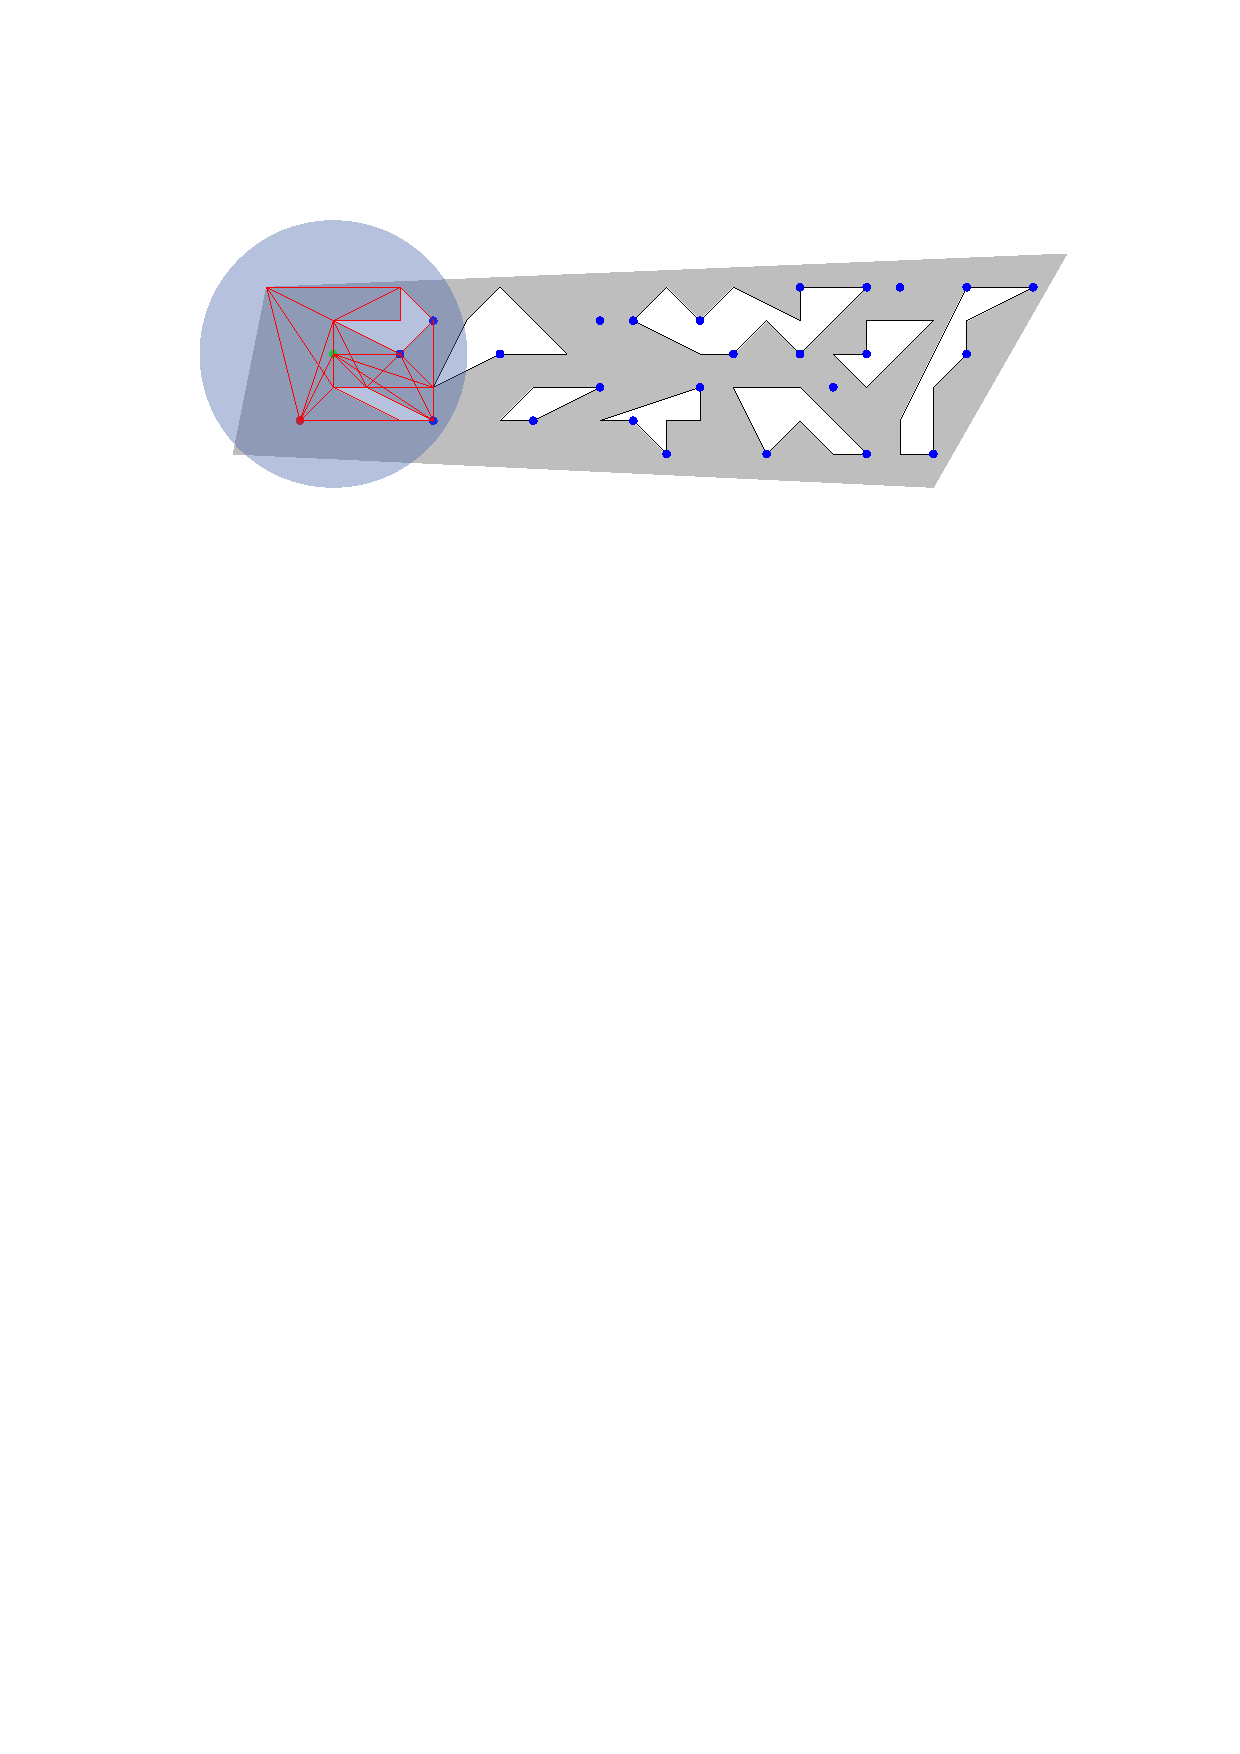
\includegraphics[page=1,height=80pt]{graphics/further_solutions.pdf}%
}%
\only<2>{%
\includegraphics[page=2,height=80pt]{graphics/further_solutions.pdf}%
}%
\end{center}

\end{frame}

\begin{frame}{Questions?}

\begin{center}
\includegraphics[page=12,height=200pt]{graphics/algo_basic.pdf}
\end{center}

\end{frame}


%\begin{frame}[t,allowframebreaks]{References}
%\bibliographystyle{apalike}
%\bibliography{references}
%\end{frame}

\end{document}
